\section{Ejercicio 7}

En este ejercicio se busca generalizar el problema anterior para N entradas, tomando como regla que si el producto de las entradas es 1 entonces la salida es 1 y si el producto de las entradas es -1 entonces la salida es -1. Se propone usar el mismo esquema de la primera arquitectura y se quiere ver como cambian los resultados frente a distintas combinaciones de cantidad de dimensión de datos de entrada N y cantidad de neuronas de la capa oculta N\'.

\begin{figure}[H]
    \centering
    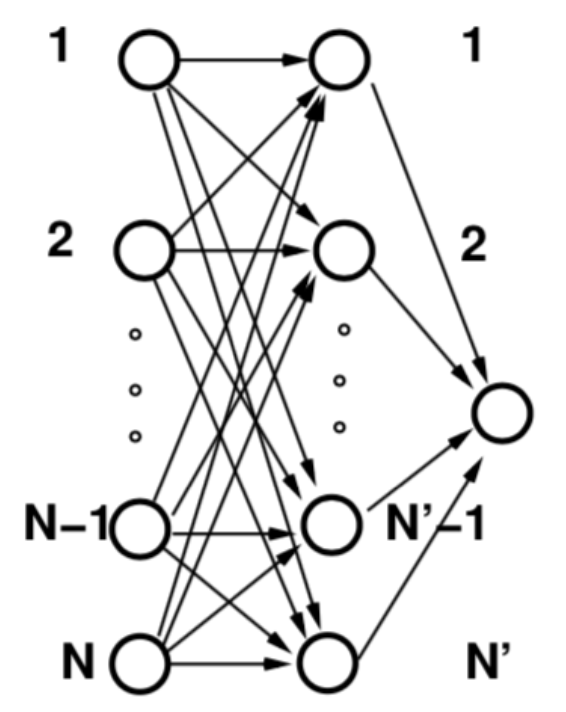
\includegraphics[width=0.3\textwidth]{image/neuronas.png}
    \caption{Problema 7: generalización de la regla XOR}
    \label{fig:my_label}
\end{figure}

Cuando se mantiene fija la dimensión de los datos de entrada y se varían las neuronas de la capa oculta, se obtienen los siguientes resultados para el accuracy y la loss:

\begin{figure}[H]
     \centering
     \begin{subfigure}[b]{0.45\textwidth}
         \centering
         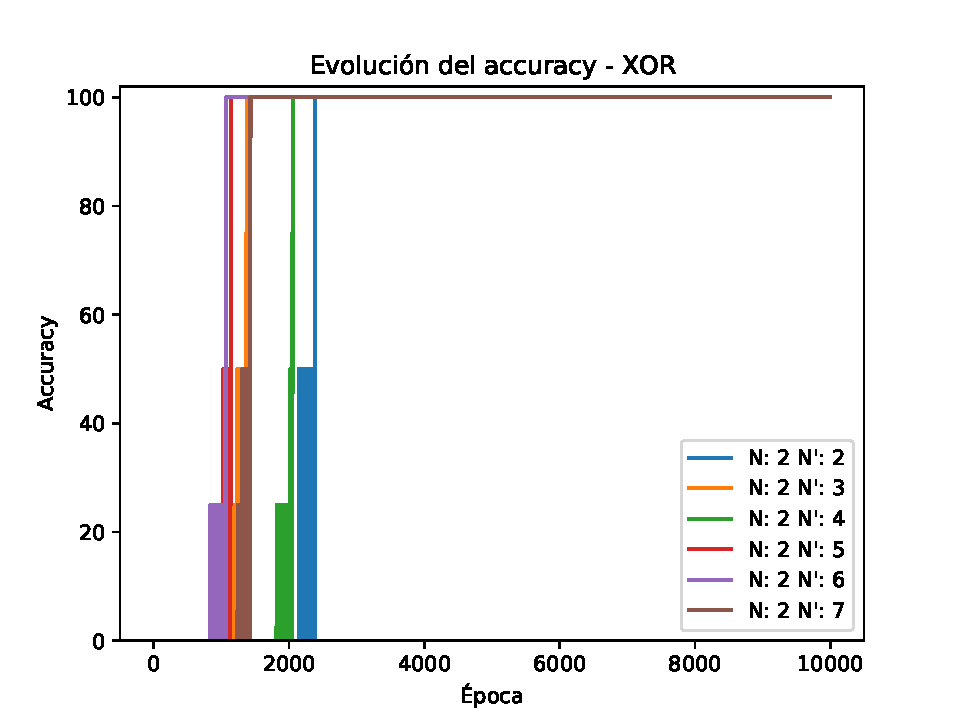
\includegraphics[width=\textwidth]{image/NvsNp_acc.pdf}
         \caption{Accuracy para el problema de aprendizaje de la regla XOR para dimensión de los datos de entrada de 2 variando la cantidad de neuronas de la capa oculta}
         \label{fig:acc6a}
     \end{subfigure}
     \hfill
     \begin{subfigure}[b]{0.45\textwidth}
         \centering
         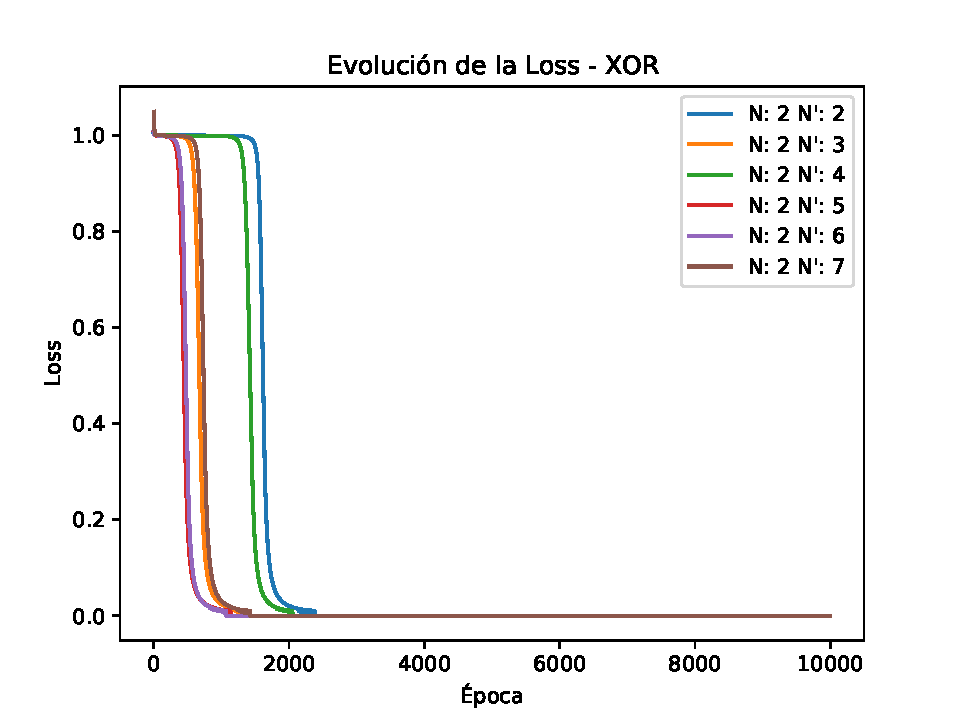
\includegraphics[width=\textwidth]{image/NvsNp_loss.pdf}
         \caption{Loss para el problema de aprendizaje de la regla XOR  para dimensión de los datos de entrada de 2 variando la cantidad de neuronas de la capa oculta}
         \label{fig:loss6a}
     \end{subfigure}
        % \caption{Resultados para la segunda arquitectura presentada para resolver el problema de la regla XOR con dos capas densas}
        % \label{fig:resu6a}
\end{figure}

Lo que se ve de estos resultados es que para la dimensión de los datos de entrada N fijos (en 2 en este caso) a medida que aumenta la cantidad de neuronas de la capa oculta $N'$ es más rápido el aprendizaje de la regla XOR. De acá surge que si uno quisiera lograr un aprendizaje más acelerado, uno preferiría usar más neuronas en las capas ocultas, aunque es claro que a mayor cantidad de neuronas, mayor es el costo computacional de este tipo de problemas.

Si ahora se mantiene fijo $N'$ (por ejemplo en 15) y se varía la dimensión de los datos de entrada, se obtienen los siguientes resultados:

\begin{figure}[H]
     \centering
     \begin{subfigure}[b]{0.45\textwidth}
         \centering
         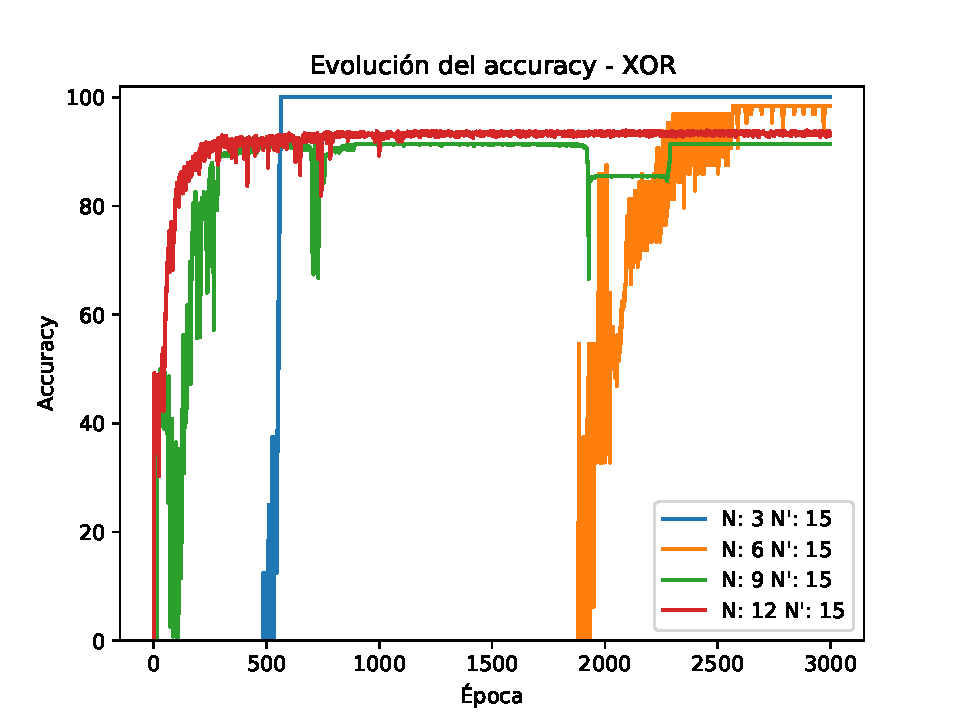
\includegraphics[width=\textwidth]{image/NvsNp_acc2.pdf}
         \caption{Accuracy para el problema de aprendizaje de la regla XOR  para dimensión de los datos de entrada de variable y con la cantidad de neuronas de la capa oculta fija en 15}
         \label{fig:acc6a}
     \end{subfigure}
     \hfill
     \begin{subfigure}[b]{0.45\textwidth}
         \centering
         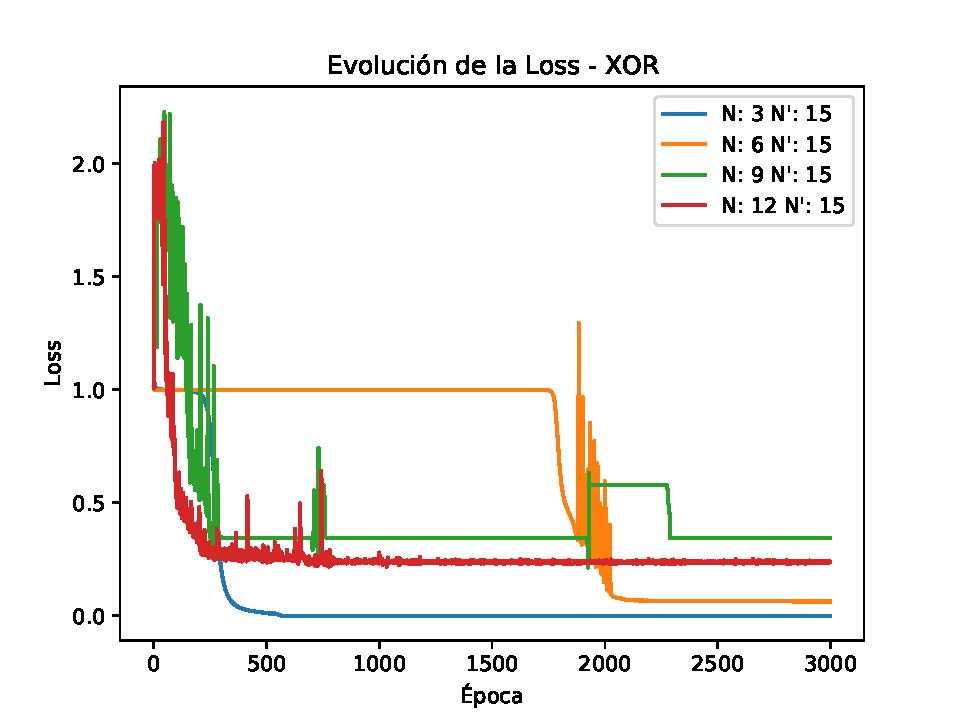
\includegraphics[width=\textwidth]{image/NvsNp_loss2.pdf}
         \caption{Loss para el problema de aprendizaje de la regla XOR  para dimensión de los datos de entrada de variable y con la cantidad de neuronas de la capa oculta fija en 15}
         \label{fig:loss6a}
     \end{subfigure}
        % \caption{Resultados para la segunda arquitectura presentada para resolver el problema de la regla XOR con dos capas densas}
        % \label{fig:resu6a}
\end{figure}

Finalmente, para el caso en que $N' << N$ se tiene que el método no logra el aprendizaje en las 3000 épocas como se ve en la siguiente figura:

\begin{figure}[H]
     \centering
     \begin{subfigure}[b]{0.45\textwidth}
         \centering
         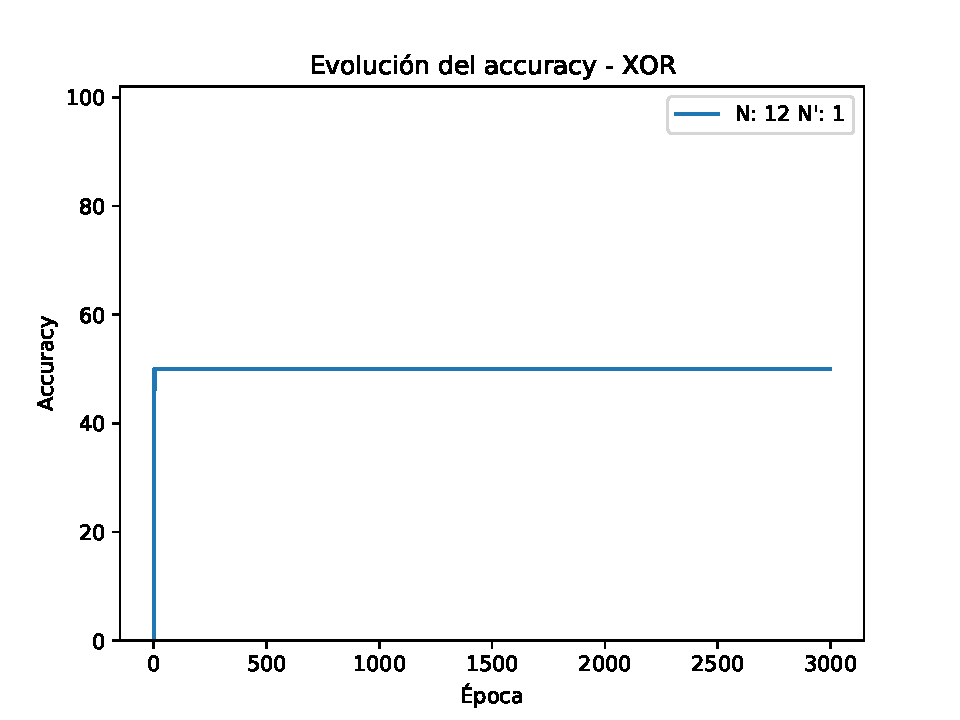
\includegraphics[width=\textwidth]{image/NvsNp_acc3.pdf}
         \caption{Accuracy para el problema de aprendizaje de la regla XOR cuando N\'<<N}
         \label{fig:acc6a}
     \end{subfigure}
     \hfill
     \begin{subfigure}[b]{0.45\textwidth}
         \centering
         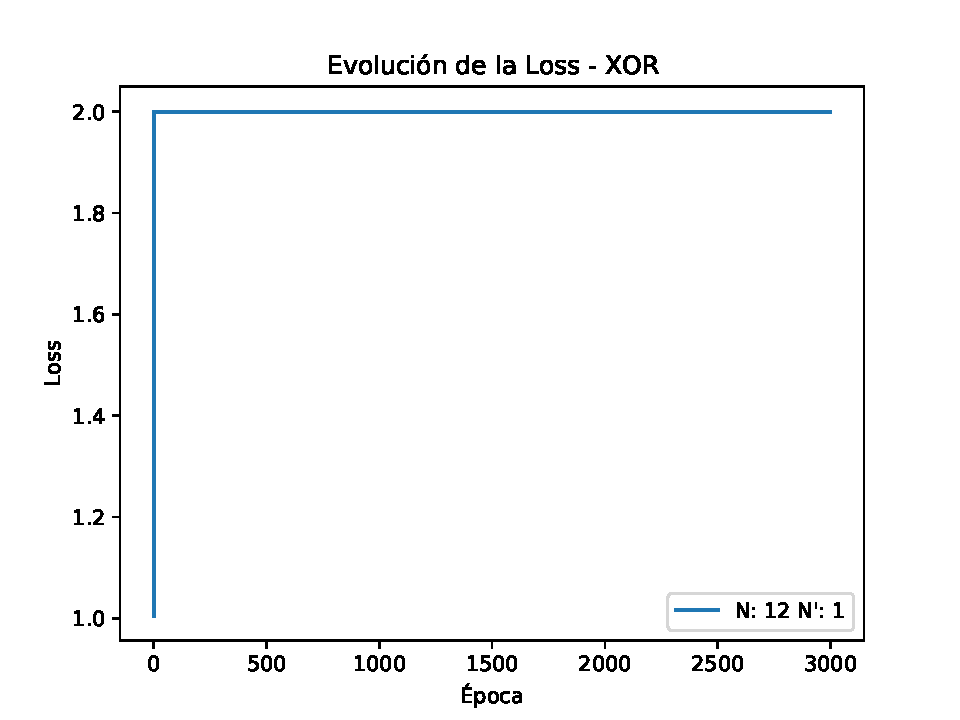
\includegraphics[width=\textwidth]{image/NvsNp_loss3.pdf}
         \caption{Loss para el problema de aprendizaje de la regla XOR cuando N\'<<N}
         \label{fig:loss6a}
     \end{subfigure}
        % \caption{Resultados para la segunda arquitectura presentada para resolver el problema de la regla XOR con dos capas densas}
        % \label{fig:resu6a}
\end{figure}